\documentclass{article}
\usepackage{tikz, comment}
\usepackage{pifont}
\usepackage{fontspec, pgfplots}
\usetikzlibrary{arrows, decorations.markings, decorations.pathreplacing}
\begin{comment}
:Title: Not defined yet
:Tags: absolute value rules;properties of equality, equation rules;equivalence properties of equality;proper subset;trichotomy
:Prob: 0.7885;0.6895;0.6087;0.5913;0.5672
:Author: Prof.Hu Ji-shan, HKUST
:Slug: No name yet

Description Here.........
\end{comment}
\begin{document}\centering 

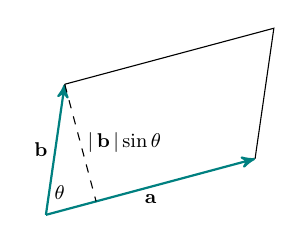
\begin{tikzpicture}[>=latex,xscale=.5*1.1, yscale=.5*1.1][font=\sf\small] 

\begin{scope}[rotate=15]
\draw[teal, thick, ->, >=stealth'] (0, 0) -- (5, 0) node[black, below, midway, pos=0.5, xshift=0, yshift=0, scale=0.8]{${\bf a}$};

\draw[teal, thick, ->, >=stealth'] (0, 0) -- (1.2, 2.8) node[black, left, midway, pos=0.5, xshift=0, yshift=0, scale=0.8]{${\bf b}$};

\draw[dashed] (1.2, 2.8) -- (1.2, 0) node[black, right, midway, pos=0.5, xshift=0, yshift=0, scale=0.8]{$|\,{\bf b} \,|\sin \theta$};

\draw[] (1.2, 2.8) --++ (5, 0) -- (5, 0);

\node[xshift=5, yshift=8, scale=0.8] at (0,0) {$\theta$};
\end{scope}

\end{tikzpicture}
\end{document}